\section{Introduction}

\subsection{Contexte}
Le pilotage de drones FPV (\textit{First Person View}) repose sur un retour vidéo en temps réel. 
Pour garantir la sécurité du vol et la réactivité du pilote, la fiabilité de la liaison radio et 
la minimisation de la latence sont absolument critiques. Actuellement, la grande majorité des retours 
vidéo commerciaux reposent sur des liaisons fonctionnant dans les bandes de fréquences de 2.4 GHz ou 
5.8 GHz. Bien que ces hautes fréquences offrent une large bande passante permettant le transfert 
de vidéos en haute définition, leur capacité de pénétration est en revanche médiocre face aux obstacles 
physiques. 

En environnement urbain, forestier ou industriel (conditions dites \textit{Non-Line-Of-Sight} ou NLOS), 
la portée de ces systèmes vidéo se trouve drastiquement réduite. À l'inverse, les protocoles opérant 
dans les bandes inférieures à 1 GHz (Sub-1 GHz, tels que TBS Crossfire ou ExpressLRS) sont devenus le 
standard industriel pour le lien de contrôle (la radiocommande) grâce à leur robustesse face 
aux obstacles, mais leur bande passante a toujours été techniquement insuffisante pour y faire transiter 
de la vidéo.

\subsection{Problématique}
Pour pallier ce manque et réunir le meilleur des deux mondes, la norme IEEE 802.11ah, également connue 
sous le nom de Wi-Fi HaLow, se présente comme une alternative prometteuse. Opérant dans la bande de 
fréquences Sub-1 GHz, elle offre une portée kilométrique et une excellente capacité à traverser les 
matériaux, tout en proposant des débits de l'ordre du Mégabit par seconde. 

Cependant, les standards Wi-Fi classiques n'ont pas été conçus à l'origine pour transporter des flux 
vidéo continus et déterministes à très faible latence. Les mécanismes natifs d'adaptation de débit 
(\textit{Rate Control}) et les retransmissions automatiques de paquets visent à garantir l'intégrité 
absolue des données au détriment du temps de livraison. Pour le vol FPV, l'attente d'une retransmission 
introduit une gigue (\textit{jitter}) et une latence totalement incompatibles avec les exigences de 
pilotage.

\subsection{Objectifs du travail de Bachelor}
L'objectif principal de ce projet est d'étudier, de concevoir et de valider de bout en bout un prototype 
de transmission vidéo exploitant les avantages physiques de la norme IEEE 802.11ah (Wi-Fi HaLow). 

Plutôt que de se limiter à la simple configuration logicielle de modules radio, l'enjeu s'est révélé être 
une véritable optimisation du système dans son ensemble. Cela implique le contournement des mécanismes 
d'acquittement réseau (diffusion unidirectionnelle), le réglage strict des pipelines de compression vidéo 
matérielle, ainsi que la mise en place d'une synchronisation physique entre les différents processeurs 
et microcontrôleurs embarqués pour éviter l'accumulation de données dans les mémoires tampons 
(\textit{buffers}).

\subsubsection{Définition du seuil d'acceptabilité et cas d'usage}
Au-delà de l'optimisation technique de la chaîne, il convient de définir un objectif de latence global 
pragmatique, aligné avec les contraintes physiques du vol en immersion. Sur une machine de type 
"freestyle" ou de course, les systèmes de transmission numériques traditionnels (opérant en 5.8 GHz) 
ciblent une latence de 20 à 30 ms (voire inférieure) pour autoriser des manœuvres très agressives.

Toutefois, l'objectif de ce travail n'est pas de concurrencer ces systèmes sur la vitesse pure, mais de 
privilégier la robustesse et la pénétration de signal en milieu complexe (conditions NLOS telles que 
l'exploration de bâtiments isolés, de forêts denses ou de tunnels). Dans ce contexte d'exploration, une 
absence de perte de liaison est préférable à une latence absolue minimale. 

Le pilotage reste parfaitement viable et sécurisant jusqu'à un seuil de latence d'environ 80 ms. 
L'objectif de ce système, une fois toutes les optimisations matérielles et logicielles appliquées, 
est donc d'atteindre ce seuil des 80 ms, qui représente une limite raisonnable au vu de la
chaîne d'acquisition matérielle grand public exploitée dans ce projet.

\subsection{Structure du document}
Ce rapport s'articule autour d'une progression logique, allant de la mise en place des fondations 
matérielles et logicielles jusqu'à l'optimisation itérative du système complet. Après une étude de 
faisabilité validant nos choix technologiques, nous détaillerons l'architecture globale retenue.
\begin{figure}[htbp]
    \centering
    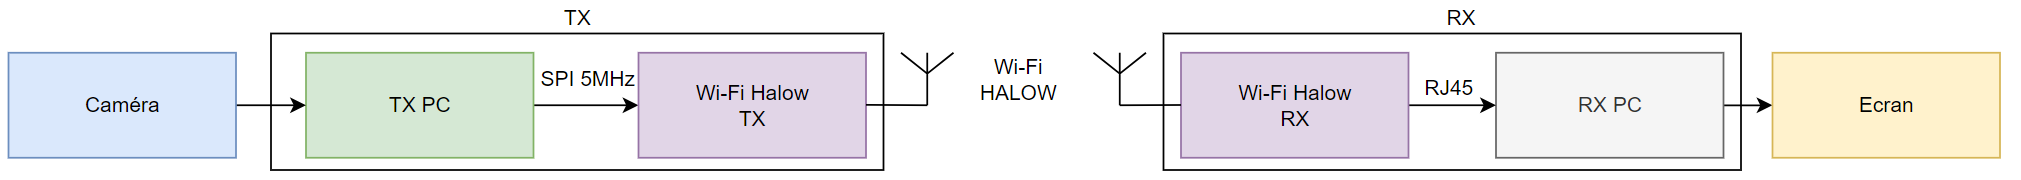
\includegraphics[width=1\textwidth]{imgs/simple_schematic.png}
    \caption{Structure globale du système}
    \label{fig:simple_schematic}
\end{figure}
\newline \newline
Après l'analyse de l'architecture globale, la première partie aborde l'implémentation spécifique du lien réseau 
Wi-Fi HaLow. 
\newline \newline
La seconde section décrit les mécanismes logiciels de capture et de traitement de la vidéo, suivis de 
l'interfaçage matériel SPI permettant d'acheminer ce flux vers le modem d'émission. 
\newline \newline
Enfin, la dernière partie est 
consacrée à la traque expérimentale de la latence et à la présentation des mesures de performances obtenues sur le 
terrain.

%\subsection{Structure du document2}
%Ce rapport s'articule autour d'une progression logique, allant de la mise en place des fondations 
%matérielles et logicielles jusqu'à la validation expérimentale du système complet. 

%\begin{figure}[htbp]
%    \centering
%    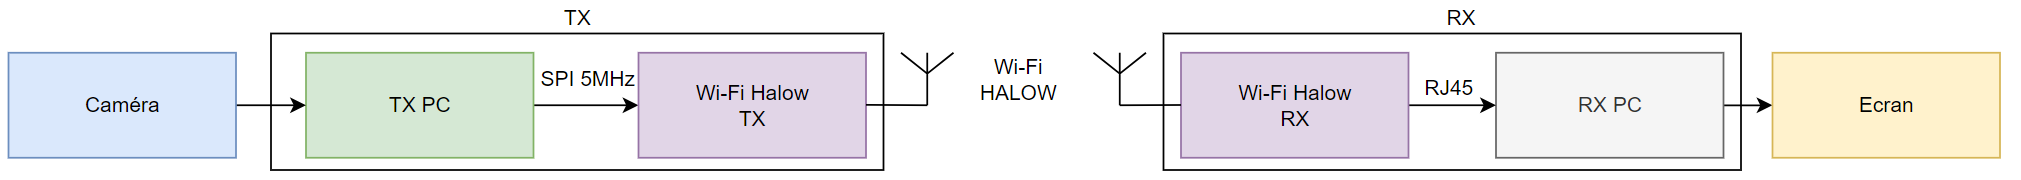
\includegraphics[width=0.85\textwidth]{imgs/simple_schematic.png}
%    \caption{Roadmap de lecture et articulations des sections du rapport}
 %   \label{fig:simple_schematic2}
%\end{figure}

%Après l'analyse de l'architecture globale, la première partie aborde l'implémentation spécifique du lien réseau 
%Wi-Fi HaLow. La seconde section décrit les mécanismes logiciels de capture et de traitement de la vidéo, suivis de 
%l'interfaçage matériel SPI permettant d'acheminer ce flux vers le modem d'émission. Enfin, la dernière partie est 
%consacrée à la traque expérimentale de la latence et à la présentation des mesures de performances obtenues sur le 
%terrain.

%\begin{figure}[htbp]
%    \centering
%    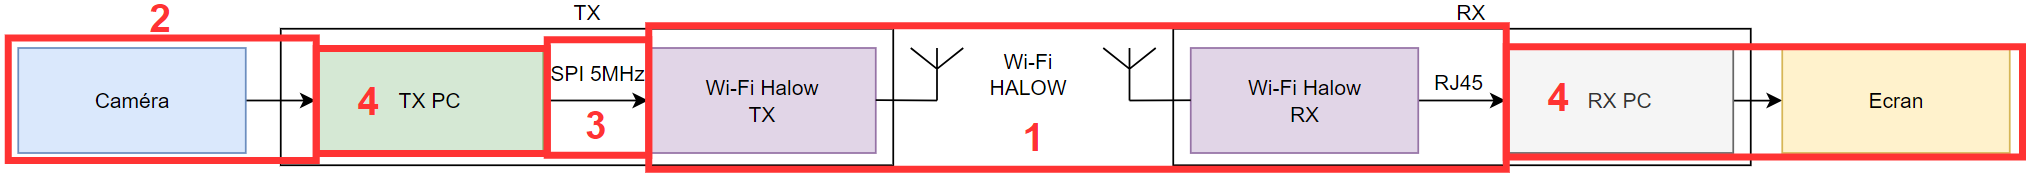
\includegraphics[width=1\textwidth]{imgs/simple_schematic_nb.png}
%    \caption{Flux logique du système : (1) Lien réseau Sub-1 GHz, (2) Capture vidéo, (3) Interfaçage SPI, (4) Plateformes de traitement TX et RX.}
%    \label{fig:roadmap_intro}
%\end{figure}